\documentclass[tikz,border=5pt]{standalone}
\usetikzlibrary{arrows,positioning, calc}

\newcommand{\numcirc}[1]{%
  \tikz[baseline=(char.base)]{
    \node[shape=circle, draw, inner sep=1pt] (char) {#1};
  }%
}

\begin{document}
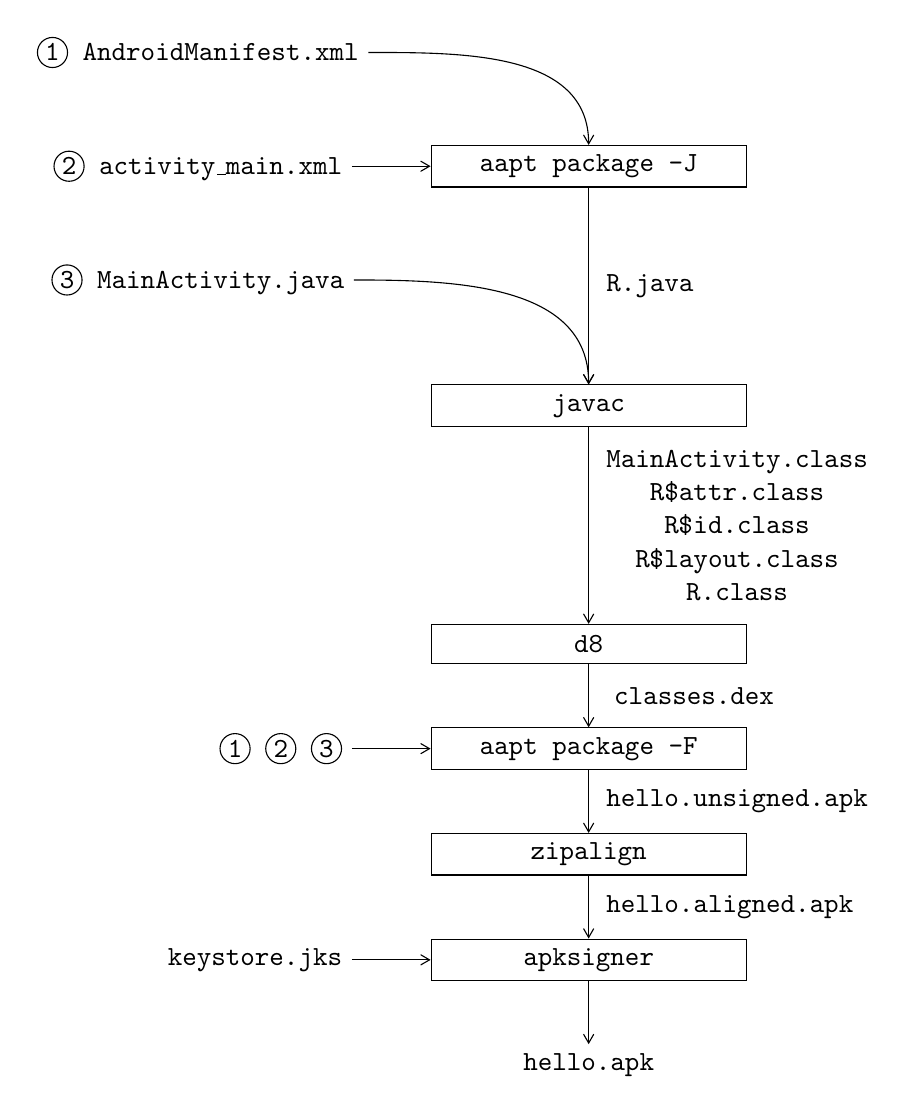
\begin{tikzpicture}[
    node/.style={draw, minimum width=4cm, minimum height=0.5cm, align=center},
    ->, >=angle 60,font=\ttfamily, node distance = 0.8cm,%draw=white,text=white
]

% Nodes
\node (manifest) {\numcirc{1} AndroidManifest.xml};
\node[below=of manifest] (xml) {\numcirc{2} activity\_main.xml};
\node[below=of xml] (java) {\numcirc{3} MainActivity.java};
\node[right=1cm of xml,node] (aaptj) {aapt package -J};
\node[below=2.5cm of aaptj,node] (javac) {javac};
\node[below=2.5cm of javac,node] (d8) {d8};
\node[below=of d8,node] (aaptf) {aapt package -F};
\node[left=1cm of aaptf] (aaptfres) {\numcirc{1} \numcirc{2} \numcirc{3} };
\node[below=of aaptf,node] (zipalign) {zipalign};
\node[below=of zipalign,node] (apksigner) {apksigner};
\node[left=1cm of apksigner] (keystore) {keystore.jks};
\node[below=of apksigner] (out) {hello.apk};

% Arrows with outputs as labels
\draw (xml) -- (aaptj);
\draw (aaptj) -- (javac) node[midway,right=1mm] {R.java};
\draw (javac) -- (d8) node[align=center,midway,right=1mm] {MainActivity.class\\R\$attr.class\\R\$id.class\\R\$layout.class\\R.class};
\draw (d8) -- (aaptf) node[midway,right=2mm] {classes.dex};
\draw (aaptf) -- (zipalign) node[midway,right=1mm] {hello.unsigned.apk};
\draw (zipalign) -- (apksigner) node[midway,right=1mm] {hello.aligned.apk};
\draw (apksigner) -- (out);
\draw (keystore) -- (apksigner);
\draw (aaptfres) -- (aaptf);

% Curved arrows on left side
\draw (java.east) to[out=0,in=90] (javac.north);
\draw (manifest.east) to[out=0, in=90] (aaptj);

\path let \p1 = (current bounding box.south west),
          \p2 = (current bounding box.north east)
      in coordinate (bbSW) at (\x1,\y1)
         coordinate (bbNE) at (\x2,\y2);

\pgfresetboundingbox
\path[use as bounding box]
  ($(bbSW)+(0mm,0mm)$) rectangle ($(bbNE)+(0mm,0mm)$);

\end{tikzpicture}
\end{document}
